\documentclass[12pt]{beamer}

\usepackage[frenchb]{babel}
\usepackage[T1]{fontenc}
\usepackage[utf8]{inputenc}
\usepackage{lmodern}% http://ctan.org/pkg/lm

\usepackage{pslatex} %pour un pdf lisible à l'écran

\usepackage{tikz} % allows to place stuff differently

\useinnertheme[shadow=true]{rounded}
\useoutertheme{infolines}
\usecolortheme{beaver}

\setbeamerfont{block title}{size={}}
\setbeamercolor{titlelike}{parent=structure,bg=white}

\title[Création d’un TPS avec le Shine Engine]{Création d’un Third-Person Shooter\\ avec le Shine Engine}
\author[Virgil MANRIQUE \hspace{2mm} Quentin GUILLIEN]{%

\includegraphics[height=14mm]{logo_shine.png} \hspace{20mm} 
\includegraphics[height=14mm]{logo-ufc.png}\\\vspace{4mm}
Virgil MANRIQUE \\ Quentin GUILLIEN}
\date{\today}


\addtobeamertemplate{frametitle}{}{%
\begin{tikzpicture}[remember picture,overlay]
\node[anchor=north east,yshift=-8pt] at (current page.north east) {
\includegraphics[height=9mm]{logo_shine.png} \hspace{1mm} 
\includegraphics[height=9mm]{logo-ufc.png}};
\end{tikzpicture}}

\LetLtxMacro\olditemize\itemize


\begin{document}

\begin{frame}
\titlepage

\end{frame}


\AtBeginSection[]
{
  \begin{frame}{Sommaire}
  \small \tableofcontents[currentsection, hideothersubsections]
  \end{frame} 
}


\renewcommand{\itemize}[1][<+(1)->]{\olditemize[#1]} %'Transition' pour les listes
\setbeamercovered{transparent} % les éléments qui ne sont pas encore atteints sont grisés

\section{Cadre du projet}

\subsection{Les Third-Person Shooter}
\begin{frame}
\frametitle{Les Third-Person Shooter}

\begin{itemize}
\item
Sous-genre des jeux de tir
\item
Vue objective de l'avatar
\end{itemize}

\end{frame}

\subsection{Les moteurs de jeu}
\begin{frame}
\frametitle{Les moteurs de jeu}

\begin{itemize}
\item
Solution logicielle haut niveau
\item
Permet la focalisation sur les mécaniques de jeu
\end{itemize}
\end{frame}

\subsection{Le Shine Engine}
\begin{frame}
\frametitle{Le Shine Engine}
\begin{itemize}
\item
Moteur de Jeu développé en C++
\item
Multi-plateforme 
\item
Dispose d'un éditeur graphique

\end{itemize}

\end{frame}



\section{Préparation}
\subsection{Les Outils}
\begin{frame}
\frametitle{Les outils}
\framesubtitle{Les indispensables}


\begin{itemize}
\item
Shine SDK
\item
Microsoft Visual Studio 2010
\item
Microsoft DirectX SDK
\item
Microsoft .NET Framework

\end{itemize}

\end{frame}
\begin{frame}
\frametitle{Les outils}
\framesubtitle{Les utiles}

\begin{itemize}
\item
GIMP
\item
XnView
\item
Git (Github)
\item
Trello
\item
\LaTeX
\end{itemize}

\end{frame}

\subsection{L'éditeur}
\begin{frame}
\frametitle{Shine Editor}
\begin{figure}
   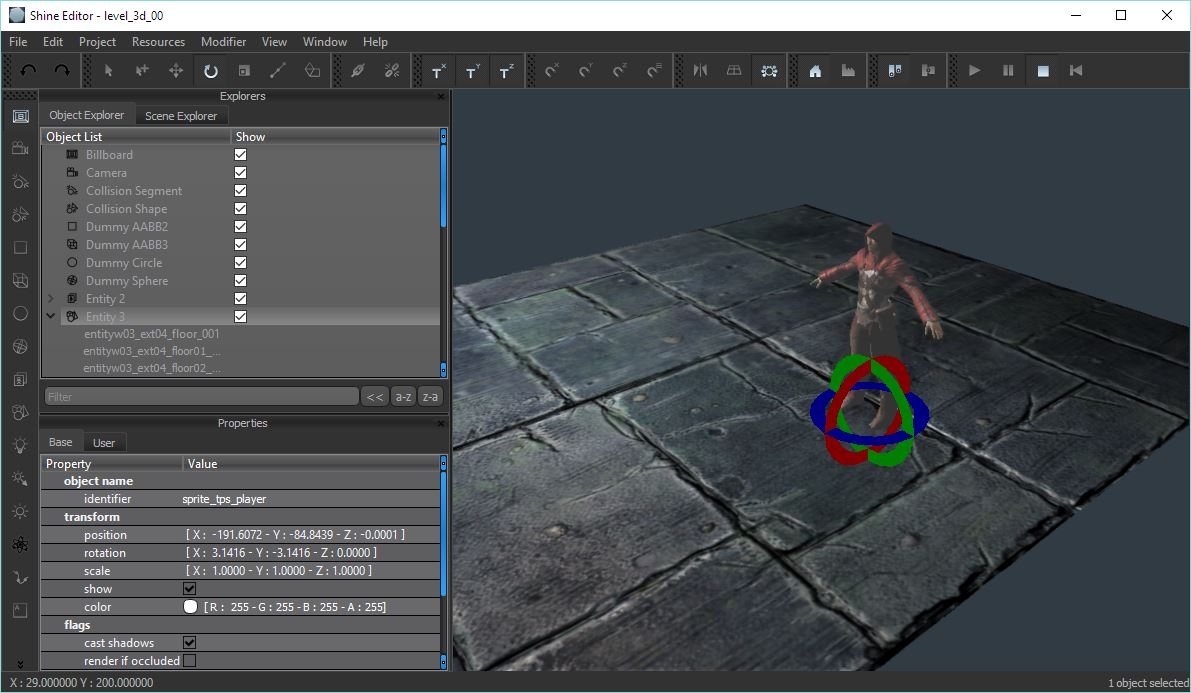
\includegraphics[width=10cm]{shine_editor.jpg}
\end{figure}
\end{frame}


\section{Réalisation}
\subsection{Plugin}
\begin{frame}
\frametitle{Plugin ou Jeu ?}
\begin{itemize}
\item
Un plugin, pas un jeu.
\item
Différences plugin / Jeu
\end{itemize}
\end{frame}

\subsection{Éléments du plugin}
\begin{frame}[t]
\frametitle{Eléments du plugins}
\begin{itemize}
\item
Personnage
\begin{itemize}
\item
Joueur
\item
Ennemi
\end{itemize}
\item
Armes
\item
Munitions
\item
Camera
\item
Gestionnaire de Collisions

\end{itemize}

\end{frame}

\subsection{Démonstration}
\begin{frame}[c]
\begin{center}
\Huge Démonstration
\end{center}


\end{frame}

\subsection{Difficultés rencontrées}
\begin{frame}
\begin{itemize}
\item
Visual Studio 2010
\item
Pas suffisamment de documentation pour Shine
\end{itemize}
\end{frame}


\setbeamertemplate{headline}{}

\begin{frame}[c]

\begin{center}
\Huge Bilan
\end{center}


\end{frame}

\begin{frame}[c]

\begin{center}
\huge Des Questions ?
\end{center}


\end{frame}




\end{document}

